\documentclass[thesis.tex]{subfiles}

\pagebreak
\appendix
\chapter{Example model output}
Some examples of the trained model's output are shown in Figures \ref{fig:rn-results-1} and \ref{fig:rn-results-2}. Ground-truth boxes are in greeen, while predicted boxes are in red.

\begin{figure}[ht!]
    \centering
    \begin{subfigure}[t]{0.45\textwidth}
        \centering
        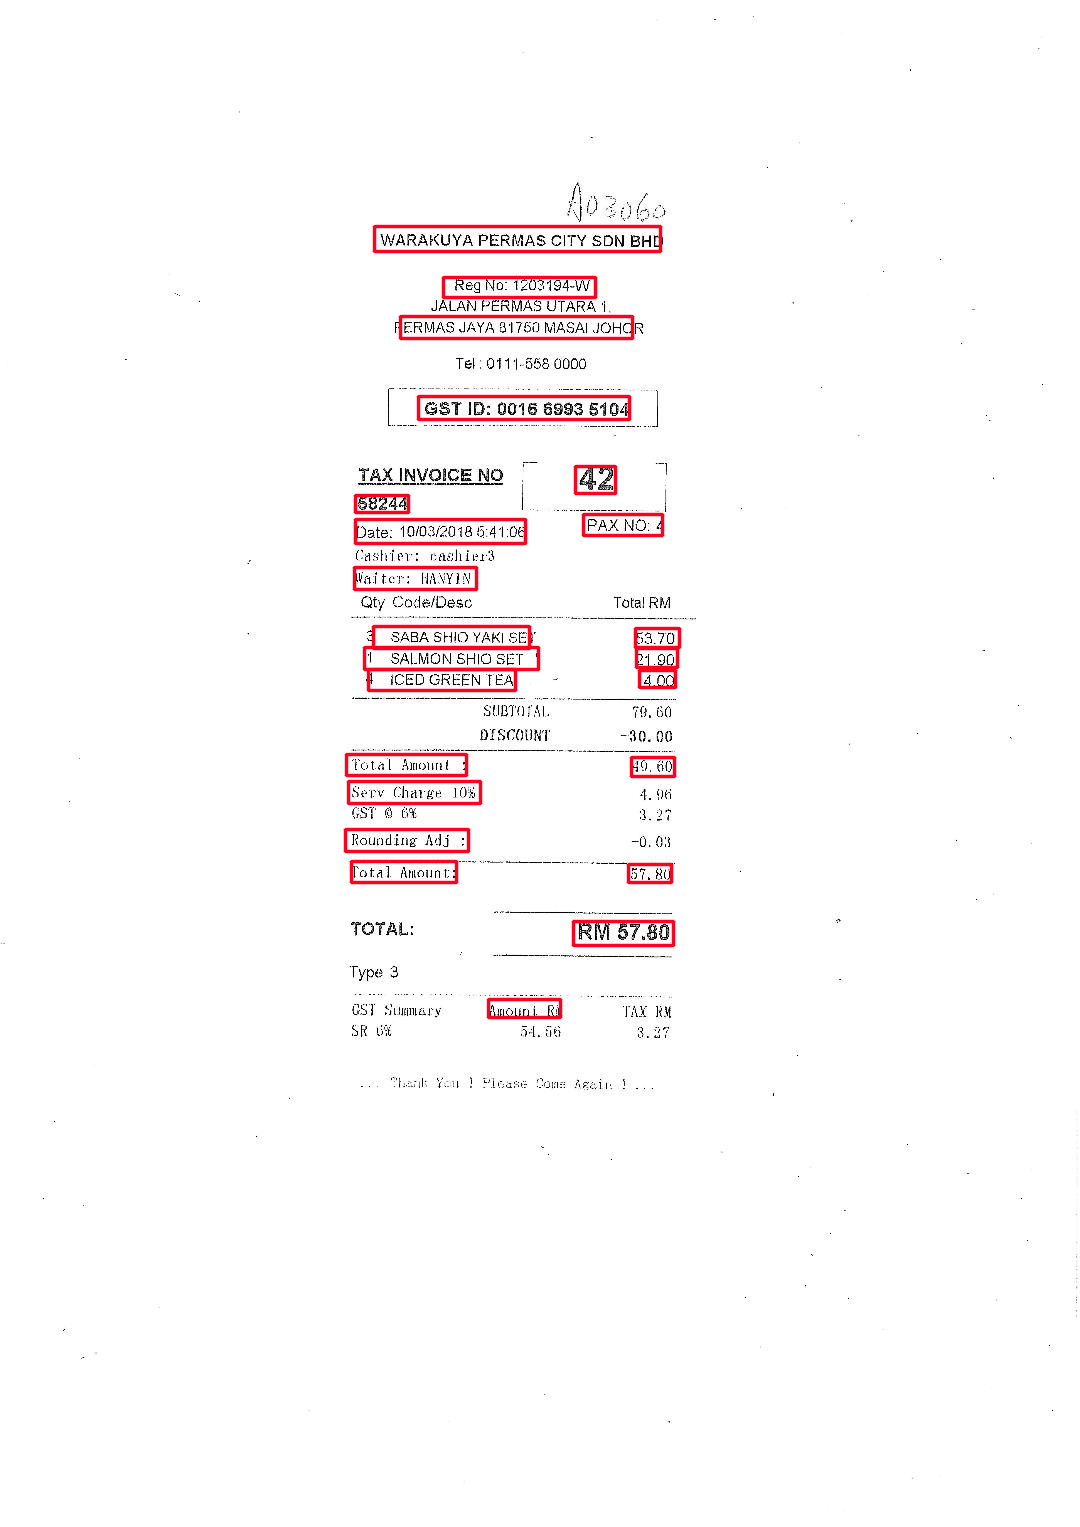
\includegraphics[width=0.45\textwidth,frame]{rn-result-4.png}
    \end{subfigure}
    \begin{subfigure}[t]{0.45\textwidth}
        \centering
        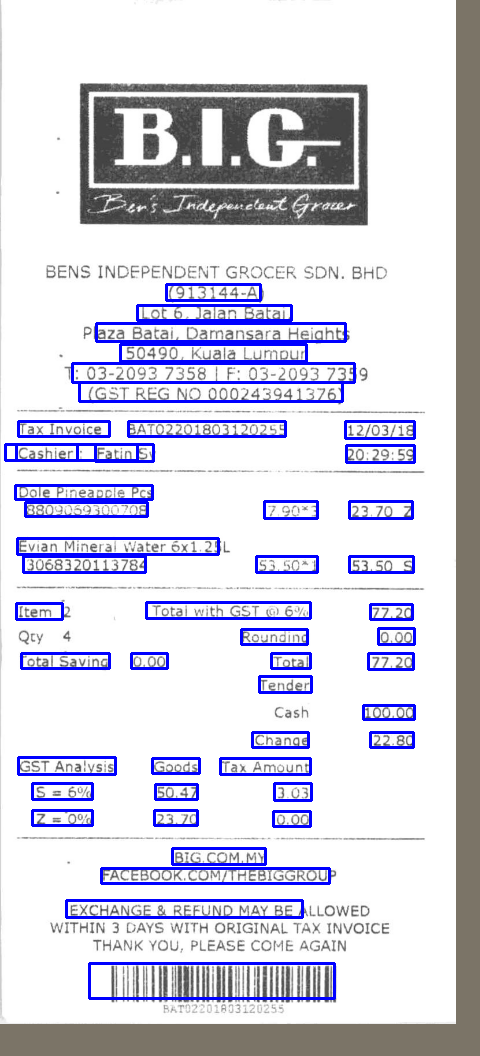
\includegraphics[width=0.45\textwidth,frame]{rn-result-2.png}
    \end{subfigure}
    \caption{RetinaNet-101-DA output on the test set (1)}
	\label{fig:rn-results-1}
\end{figure}
\FloatBarrier

\begin{figure}[ht!]
    \centering
    \begin{subfigure}[t]{0.45\textwidth}
        \centering
        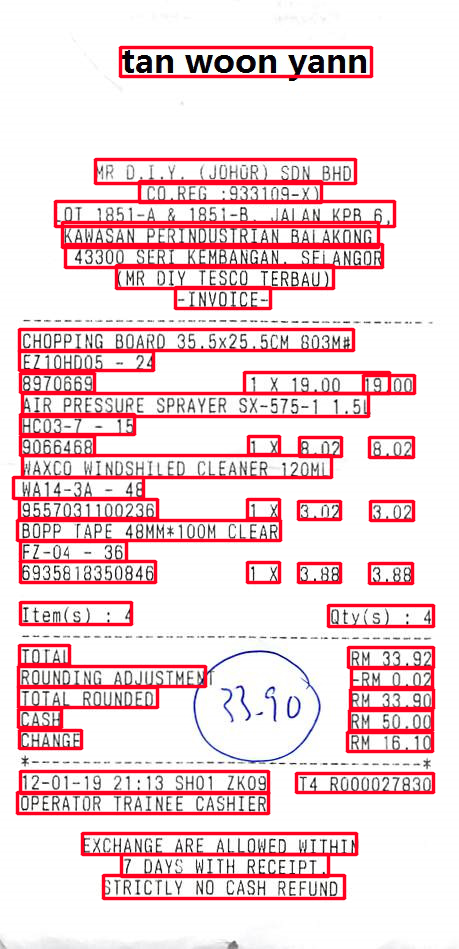
\includegraphics[width=0.45\textwidth,frame]{rn-result-3.png}
    \end{subfigure}
    \begin{subfigure}[t]{0.45\textwidth}
        \centering
        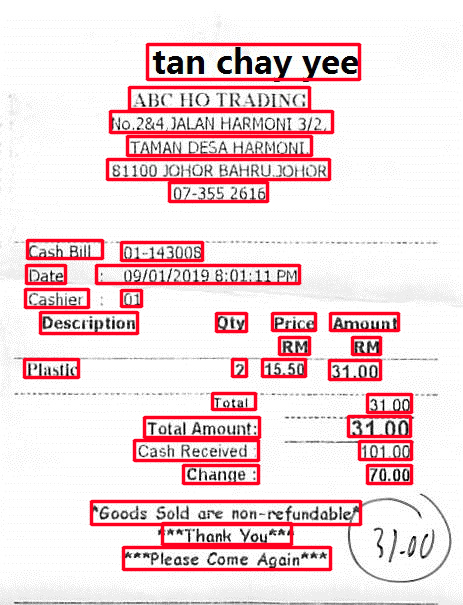
\includegraphics[width=0.45\textwidth,frame]{rn-result-1.png}
    \end{subfigure}
    \caption{RetinaNet-101-DA output on the test set (2)}
	\label{fig:rn-results-2}
\end{figure}
